% -*- TeX -*-
\documentclass[aspectratio=169]{beamer}
%\documentclass[apectratio=34]{beamer}

\usepackage{listings}

\usepackage{tikz}
\usetikzlibrary{shapes,arrows,calc}
\usetikzlibrary{decorations.pathreplacing}
\usetikzlibrary{fit,matrix}

\title{Overview of PyLith}
\subtitle{What you should have learned by reading the manual,
  etc. \ldots but didn't}
\author{Brad Aagaard}
\institute{
\includegraphics[scale=0.3]{../../logos/cig_blackfg}}
\date{June 26, 2017}

% ---------------------------------------------------- CUSTOMIZATION
%\renewcommand{\thispdfpagelabel}[1]{}
\usetheme{CIG}

% Style macros
% Style information for PyLith presentations.

% Colors
\definecolor{ltorange}{rgb}{1.0, 0.74, 0.41} % 255/188/105
\definecolor{orange}{rgb}{0.96, 0.50, 0.0} % 246/127/0

\definecolor{ltred}{rgb}{1.0, 0.25, 0.25} % 255/64/64
\definecolor{red}{rgb}{0.79, 0.00, 0.01} % 201/0/3

\definecolor{ltpurple}{rgb}{0.81, 0.57, 1.00} % 206/145/255
\definecolor{purple}{rgb}{0.38, 0.00, 0.68} % 97/1/175

\definecolor{ltblue}{rgb}{0.2, 0.73, 1.0} % 51/187/255
\definecolor{mdblue}{rgb}{0.28, 0.50, 0.80} % 72/128/205
\definecolor{blue}{rgb}{0.12, 0.43, 0.59} % 30/110/150

\definecolor{ltltgreen}{rgb}{0.7, 1.00, 0.7} % 96/204/14
\definecolor{ltgreen}{rgb}{0.37, 0.80, 0.05} % 96/204/14
\definecolor{green}{rgb}{0.23, 0.49, 0.03} % 59/125/8
  
\definecolor{dkslate}{rgb}{0.18, 0.21, 0.28} % 47/53/72
\definecolor{mdslate}{rgb}{0.45, 0.50, 0.68} % 114/127/173
\definecolor{ltslate}{rgb}{0.85, 0.88, 0.95} % 216/225/229


\newcommand{\includefigure}[2][]{{\centering\includegraphics[#1]{#2}\par}}
\newcommand{\highlight}[1]{{\bf\usebeamercolor[fg]{structure}#1}}
\newcommand{\important}[1]{{\color{red}#1}}
\newcommand{\issue}[2]{\item[Issue:] {\color{red}#1}\\{\item[Soln:] \color{blue}#2}\\[4pt]}

\setbeamercolor{alerted text}{fg=ltgreen}
\setbeamertemplate{description item}[align left]


\newcommand{\lhs}[1]{{\color{blue}#1}}
\newcommand{\rhs}[1]{{\color{red}#1}}
\newcommand{\annotateL}[2]{%
  {\color{blue}\underbrace{\color{blue}#1}_{\color{blue}\mathclap{#2}}}}
\newcommand{\annotateR}[2]{%
  {\color{red}\underbrace{\color{red}#1}_{\color{red}\mathclap{#2}}}}
\newcommand{\eqnannotate}[2]{%
  {\color{blue}%
  \underbrace{\color{black}#1}_{\color{blue}\mathclap{#2}}}}

\newcommand{\trialvec}[1][]{{\vec{\psi}_\mathit{trial}^{#1}}}
\newcommand{\trialscalar}[1][]{{\psi_\mathit{trial}^{#1}}}
\newcommand{\basisvec}[1][]{{\vec{\psi}_\mathit{basis}^{#1}}}
\newcommand{\basisscalar}[1][]{{\psi_\mathit{basis}^{#1}}}

\newcommand{\tensor}[1]{\bm{#1}}
\DeclareMathOperator{\Tr}{Tr}

\usefonttheme[onlymath]{serif}

% minted shortcuts
\newminted{cfg}{bgcolor=ltslate,autogobble,fontsize=\tiny}
\newminted{bash}{bgcolor=ltltgreen,autogobble,fontsize=\tiny}

% PyLith components
\newcommand{\pylith}[1]{{\ttfamily\color{magenta}#1}}



% --------------------------------------------------------- DOCUMENT
\begin{document}

% ------------------------------------------------------------ SLIDE
\maketitle

\logo{
\includegraphics[height=4.5ex]{../../logos/cig_blackfg}}

% ========================================================== SECTION
\section{Introduction}

% ------------------------------------------------------------ SLIDE
\begin{frame}
  \frametitle{PyLith}
  \summary{A modern, community-driven code for crustal deformation modeling}
  
  \begin{itemize}
  \item Developers
    \begin{itemize}
    \item Brad Aagaard (USGS)
    \item Matthew Knepley (Rice University)
    \item Charles Williams (GNS Science)
    \end{itemize}
  \item Combined dynamic modeling capabilities of EqSim (Aagaard) with
    the quasi-static modeling capabilities of Tecton (Williams)
  \item Use modern software engineering  to develop an open-source,
    community code 
    \begin{itemize}
    \item Modular design
    \item Testing
    \item Documentation
    \item Distribution
    \end{itemize}
  \item PyLith v1.0 was released in 2007
  \end{itemize}

  \vspace*{-2.5cm}\hspace{0.5\textwidth}\includefigure[height=3.0cm]{figs/downloads}

\end{frame}


% ------------------------------------------------------------ SLIDE
\begin{frame}
  \frametitle{Crustal Deformation Modeling}
  \summary{Elasticity problems where geometry does not change significantly}

  \vfill
  Quasi-static modeling associated with earthquakes
  \vfill

  \begin{itemize}
  \item Strain accumulation associated with interseismic deformation
    \begin{itemize}
    \item What is the stressing rate on faults X and Y?
    \item Where is strain accumulating in the crust?
    \end{itemize}
  \item Coseismic stress changes and fault slip
    \begin{itemize}
    \item What was the slip distribution in earthquake A?
    \item How did earthquake A change the stresses on faults X and Y?
    \end{itemize}
  \item Postseismic relaxation of the crust
    \begin{itemize}
    \item What rheology is consistent with observed postseismic deformation?
    \item Can aseismic creep or afterslip explain the deformation?
    \end{itemize}
  \end{itemize}
  \vfill

\end{frame}


% ------------------------------------------------------------ SLIDE
\begin{frame}
  \frametitle{Crustal Deformation Modeling}
  \summary{Elasticity problems where geometry does not change significantly}

  \vfill
  Dynamic modeling associated with earthquakes
  \vfill

  \begin{itemize}
  \item Modeling of strong ground motions
    \begin{itemize}
    \item Forecasting the amplitude and spatial variation in ground
      motion for scenario earthquakes
    \end{itemize}
  \item Coseismic stress changes and fault slip
    \begin{itemize}
    \item How did earthquake A change the stresses on faults X and Y?
    \end{itemize}
  \item Earthquake rupture behavior
    \begin{itemize}
    \item What fault constitutive models/parameters are consistent
      with the observed rupture propagation in earthquake A?
    \end{itemize}
  \end{itemize}
  \vfill

\end{frame}


% ------------------------------------------------------------ SLIDE
\begin{frame}
  \frametitle{Crustal Deformation Modeling}
  \summary{Elasticity problems where geometry does not change significantly}

  \vfill
  Volcanic deformation associated with magma chambers and/or dikes
  \begin{itemize}
  \item Inflation
    \begin{itemize}
    \item What is the geometry of the magma chamber?
    \item What is the potential for an eruption?
    \end{itemize}
  \item Eruption
    \begin{itemize}
    \item Where is the deformation occurring?
    \item What is the ongoing potential for an eruption?
    \end{itemize}
  \item Dike intrusions
    \begin{itemize}
    \item What is the geometry of the intrusion?
    \item What is the pressure change and/or amount of opening/dilatation?
    \end{itemize}
  \end{itemize}
  \vfill

\end{frame}


% ------------------------------------------------------------ SLIDE
\begin{frame}
  \frametitle{Crustal Deformation Modeling}
  \summary{Overview of workflow for typical research problem}

  \includefigure[height=7.2cm]{figs/workflow}
  
\end{frame}


% ========================================================== SECTION
\subsection{Governing Equations}

% ------------------------------------------------------------ SLIDE
\begin{frame}
  \frametitle{Governing Equations}
  \summary{}

  \vfill
  Elasticity equation
  \begin{gather}
    \sigma_{ij,j} + f_i = \rho \ddot{u} \text{ in } V, \\
    \sigma_{ij} n_j = T_i \text{ on } S_T, \\
    u_i = u_i^0 \text{ on } S_u, \text{ and } \\
    R_{ki}(u^{+}_i - u^{-}_i) = d_k \text{ on } S_f.
  \end{gather}
  Multiply by weighting function and integrate over the volume,
  \begin{equation}
    -\int_V (\sigma_{ij,j} + f_i - \rho \ddot{u}_i) \phi_i \, dV = 0
  \end{equation}
  After some algebra,
  \begin{equation}
    -\int_V \sigma_{ij} \phi_{i,j} \, dV 
    + \int_{S_T} T_i \phi_i\, dS
    + \int_V f_i \phi_i \, dV 
    - \int_V \rho \ddot{u}_i \phi_i \, dV = 0
  \end{equation}
  \vfill
  
\end{frame}


% ------------------------------------------------------------ SLIDE
\begin{frame}
  \frametitle{Discretize Domain Using Finite Elements}
   \summary{PyLith v2.0.0 and later use interpolated meshes}
 
   \begin{center}
     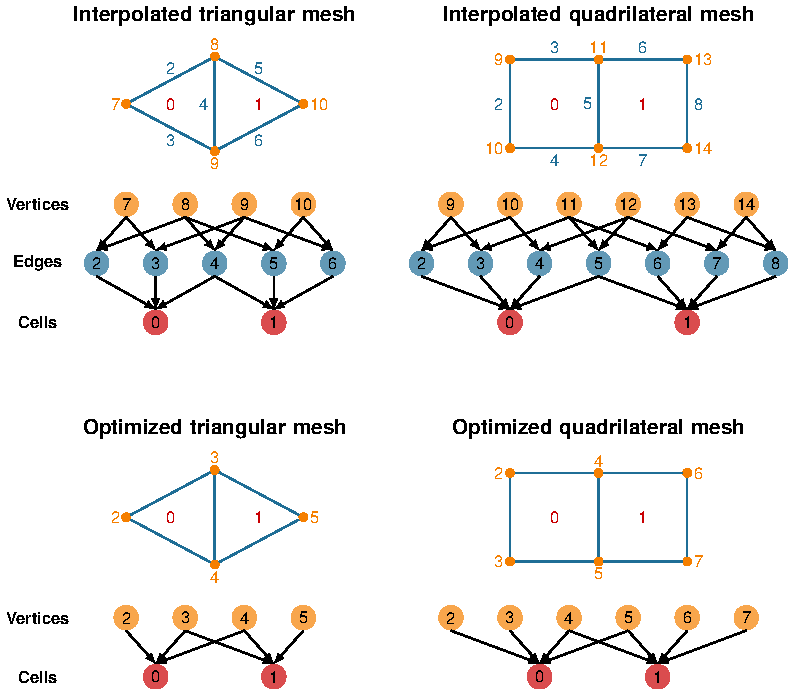
\includegraphics[height=7.0cm]{figs/meshtopology}
   \end{center}
   
 \end{frame}
 

% ========================================================== SECTION
\section{Using PyLith}

% ------------------------------------------------------------ SLIDE
\begin{frame}
  \frametitle{Overview of PyLith Workflow}
  \summary{}

  \includefigure[height=7.2cm]{figs/runpylith}
\end{frame}

% ------------------------------------------------------------ SLIDE
\begin{frame}
  \frametitle{PyLith as a Hierarchy of Components}
  \summary{Components are the basic building blocks}

  \begin{minipage}{0.53\textwidth}
    \begin{itemize}
    \item Separate functionality into discrete modules (components)
    \item Alternative implementations use the same interfaces to allow plug-n-play
    \item Top-level interfaces in Python with computational code in C++
      \begin{itemize}
      \item Python dynamic typing permits adding new modules at runtime.
      \item Users can add functionality without modifying the PyLith code.
      \end{itemize}
    \end{itemize}
  \end{minipage}\hfill
  \begin{minipage}{0.43\textwidth}
    \includefigure[height=5cm]{figs/component}
  \end{minipage}

\end{frame}

% ------------------------------------------------------------ SLIDE
\begin{frame}[fragile]
  \frametitle{Parameter Files}
  \summary{Simple syntax for specifying parameters for properties and components}

\begin{cfg}
# Syntax
<h>[pylithapp.COMPONENT.SUBCOMPONENT]</h> ; Inline comment
<f>COMPONENT</f> = OBJECT
<p>PARAMETER</p> = VALUE

# Example
<h>[pylithapp.mesh_generator]</h> ; Header indicates path of mesh_generator in hierarchy
<f>reader</f> = pylith.meshio.MeshIOCubit ; Use mesh from CUBIT/Trelis
<p>reader.filename</p> = mesh_quad4.exo ; Set filename of mesh.
<p>reader.coordsys.space_dim</p> = 2 ; Set coordinate system of mesh.

<h>[pylithapp.problem.solution_outputs.output]</h> ; Set output format
<f>writer</f> = pylith.meshio.DataWriterHDF5
<p>writer.filename</p> = axialdisp.h5

<h>[pylithapp.problem]</h>
<f>bc</f> = [x_neg, x_pos, y_neg] ; Create array of boundary conditions
<f>bc.x_neg</f> = pylith.bc.DirichletTimeDependent ; Set type of boundary condition
<f>bc.x_pos</f> = pylith.bc.DirichletTimeDependent
<f>bc.y_neg</f> = pylith.bc.DirichletTimeDependent

<h>[pylithapp.problem.bc.x_pos]</h> ; Boundary condition for +x
<p>constrained_dof</p> = [0] ; Constrain x DOF
<p>label</p> = edge_xpos ; Name of nodeset from CUBIT/Trelis
<f>db_auxiliary_fields</f> = spatialdata.spatialdb.SimpleDB ; Set type of spatial database
<p>db_auxiliary_fields.label</p> = Dirichlet BC +x edge
<p>db_auxiliary_fields.iohandler.filename</p> = axial_disp.spatialdb ; Filename for database
\end{cfg}

\end{frame}

% ------------------------------------------------------------ SLIDE
\begin{frame}
  \frametitle{Parameters Graphical User-Interface}
  \summary{{\tt cd parametersgui; ./pylith\_paramviewer}}

  \includefigure[height=8.5cm]{figs/paramgui_snapshot}

\end{frame}

% ------------------------------------------------------------ SLIDE
\begin{frame}
  \frametitle{Spatial Databases}
  \summary{User-specified field/value in space for properties and BC values.}

  \begin{itemize}
 \item Examples
    \begin{itemize}
    \item Uniform value for Dirichlet BC (0-D)
    \item Piecewise linear variation in tractions for Neumann BC (1-D)
    \item SCEC CVM-H seismic velocity model (3-D)
    \end{itemize}
  \item Generally independent of discretization for problem
  \item Available spatial databases
    \begin{description}
    \item[UniformDB] Optimized for uniform value
    \item[SimpleDB] Arbitrarily distributed points for variations in 0-D, 1-D, 2-D, or 3-D
    \item[SimpleGridDB] Logically gridded points for variations in 0-D, 1-D, 2-D, or 3-D
    \item[SCECCVMH] SCEC CVM-H seismic velocity model v5.3
    \item[ZeroDispDB] Special case of UniformDB
    \end{description}
 \end{itemize}

\end{frame}

% ------------------------------------------------------------ SLIDE
\begin{frame}
  \frametitle{PyLith Design: Focus on Geodynamics}
  \summary{Leverage packages developed by computational scientists}

  \includefigure[height=7.0cm]{figs/packages}

\end{frame}

% ------------------------------------------------------------ SLIDE
\begin{frame}
  \frametitle{PyLith Development Follows CIG Best Practices}
  \summary{\href{https://github.com/geodynamics/best\_practices}{github.com/geodynamics/best\_practices}}

  \begin{itemize}
  \item Version Control
    \begin{itemize}
    \item New features are added in separate branches.
    \item Use 'master' branch as stable development branch.
    \end{itemize}
  \item Coding
    \begin{itemize}
    \item User-friendly specification of parameters at runtime.
    \item Development plan, updated annually.
    \item Users can add features or alternative implementations without modifying code.
    \end{itemize}
  \item Portability
    \begin{itemize}
    \item Build procedure is independent of compilers and optimization flags.
    \item Multiple builds (debug/optimized) from same source.
    \end{itemize}
  \item Documentation and User Workflow
    \begin{itemize}
    \item Extensive example suite with varying levels of complexity.
    \item Changing simulation parameters does not require rebuilding.
    \item Displays version information via {\tt --version} command line argument.
    \end{itemize}
  \end{itemize}

\end{frame}

% ------------------------------------------------------------ SLIDE
\begin{frame}
  \frametitle{Development Tools}
  \summary{Leverage open-source tools for efficient code development.}

  \begin{description}
  \item[GitHub] Code repository supporting simultaneous, independent implementation of new features.
  \item[Doxygen] Document parameters and purpose of every object and its functions.
  \item[CppUnit] Test nearly every function in code during development.
  \item[Travis CI \& Jenkins] Run tests when code is committed to repository.
  \item[gcov] Records which lines of code tests cover.
  \end{description}

\end{frame}

% ------------------------------------------------------------ SLIDE
\begin{frame}
  \frametitle{Testing}
  \summary{Multiple levels of testing facilitates identifying bugs at origin.}

  \begin{description}
  \item[unit tests] Serial testing at level of single and multiple functions.
  \item[full-scale tests] Serial and parallel pass/fail tests of full problems using Method of Manufactured Solutions.
  \item[benchmarks] Serial and parallel tests for code comparisons, etc.
  \end{description}

\end{frame}

% ------------------------------------------------------------ SLIDE
\begin{frame}
  \frametitle{PyLith Current Release: v2.2.1 (Jun 25, 2017)}
  \summary{Same feature as v2.2.0, just new examples and bugfixes}

  \begin{itemize}
  \item Time integration schemes and elasticity formulations
    \begin{itemize}
    \item Implicit for quasistatic problems (neglect inertial terms)
      \begin{itemize}
      \item Infinitesimal strains
      \item Small strains
      \end{itemize}
    \item Explicit for dynamic problems
      \begin{itemize}
      \item Infinitesimal strains
      \item Small strains
      \item Numerical damping via viscosity
     \end{itemize}
    \end{itemize}
  \item Bulk constitutive models (2-D and 3-D)
    \begin{itemize}
    \item Elastic model 
    \item Linear Maxwell viscoelastic models
    \item Generalized Maxwell viscoelastic models
    \item Power-law viscoelastic model
    \item Drucker-Prager elastoplastic model
    \end{itemize}
 \end{itemize}

\end{frame}


% ------------------------------------------------------------ SLIDE
\begin{frame}
  \frametitle{Features in PyLith v2.2 (cont.)}
  \summary{}

  \begin{itemize}
  \item Boundary and interface conditions
    \begin{itemize}
    \item Time-dependent Dirichlet boundary conditions
    \item Time-dependent Neumann (traction) boundary conditions
    \item Absorbing boundary conditions
    \item Kinematic (prescribed slip) fault interfaces w/multiple ruptures
    \item Dynamic (friction) fault interfaces
    \item Fault interfaces with T intersections
    \item Time-dependent point forces
    \item Gravitational body forces
    \end{itemize}
  \item Fault constitutive models
    \begin{itemize}
    \item Static friction
    \item Linear slip-weakening
    \item Linear time-weakening
    \item Dieterich-Ruina rate and state friction w/ageing law
   \end{itemize}
 \end{itemize}

\end{frame}


% ------------------------------------------------------------ SLIDE
\begin{frame}
  \frametitle{Features in PyLith v2.2 (cont.)}
  \summary{}

  \begin{itemize}
  \item Automatic and user-controlled time stepping
  \item Ability to specify initial stress/strain state
  \item Importing meshes
    \begin{itemize}
    \item LaGriT: GMV/Pset
    \item CUBIT/Trelis: Exodus II
    \item ASCII: PyLith mesh ASCII format (intended for toy problems only)
    \end{itemize}
  \item Output: VTK and HDF5 files
    \begin{itemize}
    \item Solution over volume
    \item Solution over surface boundary
    \item Solution interpolated to user-specified points w/station names
    \item State variables (e.g., stress and strain) for each material
    \item Fault information (e.g., slip and tractions)
    \end{itemize}
 \end{itemize}
  
\end{frame}


% ------------------------------------------------------------ SLIDE
\begin{frame}
  \frametitle{Features in PyLith v2.2 (cont.)}
  \summary{}

  \begin{itemize}
  \item Automatic conversion of units for all parameters
  \item Parallel uniform global refinement
  \item PETSc linear and nonlinear solvers
    \begin{itemize}
    \item Custom preconditioner with algebraic multigrid solver
    \end{itemize}
  \item Output of simulation progress estimates runtime
 \end{itemize}
  
\end{frame}


% ========================================================== SECTION
\subsection{Fault Implementation}

% ------------------------------------------------------------ SLIDE
\begin{frame}[fragile]
  \frametitle{Fault Interface}
  \summary{Fault tractions couple deformation across interface}

  \includefigure[height=7.0cm]{figs/domaindecomp}

\end{frame}


% ------------------------------------------------------------ SLIDE
\begin{frame}
  \frametitle{Implementation: Fault Interfaces}
   \summary{Use zero volume/area cohesive cells to control fault behavior}
 
   \includefigure[height=6.2cm]{figs/cohesivecells}
   \vfill
   See Aagaard, Knepley, and Williams, JGR, 2013
   \href{http://dx.doi.org/10.1002/jgrb.50217}{doi:
     10.1002/jgrb.50217} for more information.
 \end{frame}
 

% ------------------------------------------------------------ SLIDE
\begin{frame}[fragile]
  \frametitle{Fault Implementation: Governing Equations}
  \summary{Terms in governing equation associated with fault}

  \begin{itemize}
  \item Tractions on fault surface are analogous to boundary tractions
    \tikz{
      \matrix [matrix of nodes, ampersand replacement=\&] {
      \node {$ \displaystyle \ldots $}; \&
      \node [below delimiter=\}] {$ \displaystyle + \int_{S_T} \vec{\phi} \cdot \vec{T} \, dS$}; \&
      \node [below delimiter=\}] {$ \displaystyle - \int_{S_{f^+}} \vec{\phi} \cdot \vec{l} \, dS$}; \&
      \node [below delimiter=\}] {$ \displaystyle + \int_{S_{f^-}} \vec{\phi} \cdot \vec{l} \, dS$}; \&
      \ldots = 0 \\
      \& \node {Neumann BC}; \& 
      \node {Fault +}; \&
      \node {Fault -}; \& \\
    };
}
  \item Constraint equation relates slip to relative displacement
    \tikz{
      \matrix [matrix of nodes, ampersand replacement=\&] {
        \node {$ \displaystyle \int_{S_f} \vec{\phi} \cdot ($}; \&
        \node [below delimiter=\}] {$\displaystyle\vec{d}$}; \&
        \node {$ \displaystyle - $}; \&
        \node [below delimiter=\}] {$ \displaystyle (\vec{u}_{+} - \vec{u}_{-}) $}; \&
        \node {$ \displaystyle ) dS = 0 $}; \\
        \& Slip \& \& Relative Disp. \& \\
    };
}
  \end{itemize}

\end{frame}


% ------------------------------------------------------------ SLIDE
\begin{frame}
  \frametitle{Fault Slip Implementation}
  \summary{Use Lagrange multipliers to specify slip}

  \begin{itemize}
  \item System without cohesive cells
    \begin{itemize}
    \item Conventional finite-element elasticity formulation
      \begin{equation}
        \underbar{A} \vec{u} = \vec{b} \nonumber
      \end{equation}
    \item Fault slip associated with relative displacements across fault
      \begin{equation}
        \underbar{C} \vec{u} = \vec{d} \nonumber
      \end{equation}
    \end{itemize}
  \item System with Lagrange multiplier constraints for fault slip
    \begin{equation}
      \left( \begin{array}{cc}
          \underbar{A} & \underbar{C}^T\\
          \underbar{C} & 0
        \end{array} \right)
      \left( \begin{array}{c}
          \vec{u}\\
          \vec{l}
        \end{array}\right)
      =
      \left( \begin{array}{c}
          \vec{b}\\
          \vec{d}
        \end{array} \right)
      \nonumber
    \end{equation}
  \item Prescribed (kinematic) slip\\
    Specify fault slip ($\vec{d}$) and solve for Lagrange multipliers ($\vec{l}$)
  \item Spontaneous (dynamic) slip\\
    Adjust fault slip to be compatible with fault constitutive model
\end{itemize}
  
\end{frame}


% ------------------------------------------------------------ SLIDE
\begin{frame}
  \frametitle{Implementing Fault Slip with Lagrange multipliers}
 
 \begin{itemize}
 \item Advantages
   \begin{itemize}
   \item Fault implementation is local to cohesive cell
   \item Solution includes tractions generating slip (Lagrange multipliers)
   \item Retains block structure of matrix, including symmetry
   \item Offsets in mesh mimic slip on natural faults
   \end{itemize}
 \item Disadvantages 
   \begin{itemize}
   \item Cohesive cells require adjusting topology of finite-element
     mesh
   \item Scalable preconditioner/solver is more complex
  \end{itemize}
 \end{itemize}
  
\end{frame}



% ========================================================== SECTION
\section{CUBIT/Trelis}
\subsection{General}

% ------------------------------------------------------------ SLIDE
\begin{frame}
  \frametitle{Mesh Generation Tips}
  \summary{There is no silver bullet in finite-element mesh generation}
 
  \begin{itemize}
  \item Hex/Quad versus Tet/Tri
    \begin{itemize}
    \item Hex/Quad are slightly more accurate and faster
    \item Tet/Tri easily handle complex geometry
    \item Easy to vary discretization size with Tet, Tri, and Quad cells
    \item There is no easy answer\\
      For a given accuracy, a finer resolution Tet mesh that varies
      the discretization size in a more optimal way {\bf\it might} run
      faster than a Hex mesh
    \end{itemize}
  \item Check and double-check your mesh
    \begin{itemize}
    \item Were there any errors when running the mesher?
    \item Are the boundaries, etc marked correctly for your BC?
    \item Check mesh quality (aspect ratio should be close to 1)
    \end{itemize}
  \end{itemize}

\end{frame}


% ------------------------------------------------------------ SLIDE
\begin{frame}
  \frametitle{CUBIT/Trelis Workflow}
  \summary{}
 
  \begin{enumerate}
  \item Create geometry
    \begin{enumerate}
    \item Construct surfaces from points, curves, etc or basic shapes
    \item Create domain and subdivide to create any interior surfaces
      \begin{itemize}
      \item Fault surfaces must be interior surfaces (or a subset) that completely divide domain
      \item Need separate volumes for different constitutive {\em models, not parameters}
      \end{itemize}
    \end{enumerate}
  \item Create finite-element mesh
    \begin{enumerate}
    \item Specify meshing scheme
    \item Specify mesh sizing information
    \item Generate mesh
    \item Smooth to fix any poor quality cells
    \end{enumerate}
  \item Create nodesets and blocks
    \begin{enumerate}
    \item Create block for each constitutive model
    \item Create nodeset for each BC and fault
    \item \highlight{Create nodeset for buried fault edges}
    \item Create nodeset for ground surface for output (optional)
    \end{enumerate}
  \item Export mesh in Exodus II format ({\tt .exo} files)
  \end{enumerate}

\end{frame}


% ------------------------------------------------------------ SLIDE
\begin{frame}
  \frametitle{CUBIT/Trelis Issues}
  \summary{Keep in mind the scales of the observations you are modeling}
 
  \begin{itemize}
  \item Topography/bathymetry
    \begin{itemize}
    \item Ignore topography/bathymetry unless you know it matters
    \item For rectilinear grid, create UV net surface
    \item Convert triangular facets to UV net surface via mapped mesh
    \end{itemize}
  \item Fault surfaces
    \begin{itemize}
    \item Building surfaces from contours is usually easiest
    \item Include features at the resolution that matters
    \end{itemize}
  \item Performance
    \begin{itemize}
    \item Number of points in spline curves/surfaces has huge affect
      on mesh generation runtime
    \item CUBIT/Trelis do not run in parallel
    \item Use uniform global refinement in PyLith for large sims ($>$10M cells) 
    \end{itemize}
  \end{itemize}

\end{frame}


% ------------------------------------------------------------ SLIDE
\begin{frame}
  \frametitle{CUBIT/Trelis Best Practices}
  \summary{}
 
  \begin{description}
    \issue{Changes in geometry cause changes in object ids} {Name objects and use
      APREPRO or Python to eliminate hardwired ids wherever possible}
    \issue{Splines with many points slows down operations}{Reduce the
      number of points per spline}
    \issue{Surfaces meet in small angles creating distorted
      cells}{Trim geometry to eliminate features smaller than cell
      size}
    \issue{Difficulty meshing complex geometry with Hex cells}{Use
      Tet cells even if it requires a finer mesh}
    \issue{Hex mesh over-samples parts of the
      domain}{Use Tet mesh and vary discretization within domain}
    \issue{Extended surfaces create very complex geometry}{Subdivide
      geometry before webcutting to eliminate overly complex geometry}
  \end{description}

\end{frame}


% ========================================================== SECTION
\section{Troubleshooting}
\subsection{General}

% ------------------------------------------------------------ SLIDE
\begin{frame}
  \frametitle{General Numerical Modeling Tips}
  \summary{Start simple and progressively add complexity and increase
    resolution}
  
  \begin{itemize}
  \item \highlight{Start in 2-D, if possible, and then go to 3-D}
    \begin{itemize}
    \item Much smaller problems $\Rightarrow$ much faster turnaround
    \item Start with an exact solver
    \item Experiment with meshing, boundary conditions, solvers, etc
    \item Keep in mind how physics differs from 3-D
    \end{itemize}
  \item \highlight{Start with coarse resolution and then increase resolution}
    \begin{itemize}
    \item Much smaller problems $\Rightarrow$ much faster turnaround
    \item Start with an exact solver
    \item Experiment with meshing, boundary conditions, solvers, etc.
    \item Increase resolution until solution resolves features of interest
      \begin{itemize}
      \item Resolution will depend on spatial scales in BC, initial
        conditions, deformation, and geologic structure
      \item Is geometry of domain important? At what resolution?
      \item Displacement field is integral of strains/stresses
      \item Resolving stresses/strains requires fine resolution simulations
      \end{itemize}
    \end{itemize}
  \item \highlight{Use your intuition and analogous solutions to check
      your results!}
  \end{itemize}
  
\end{frame}


% ========================================================== SECTION
\subsection{PyLith}

% ------------------------------------------------------------ SLIDE
\begin{frame}
  \frametitle{PyLith Tips}
  \summary{}
 
  \begin{itemize}
  \item \highlight{Read the PyLith User Manual}
  \item \highlight{Do not ignore error messages and warnings!}
  \item Use an example/benchmark as a starting point
  \item Quasi-static simulations
    \begin{itemize}
    \item Start with a static simulation and then add time dependence
    \item \highlight{Check that the solution converges at every time step}
    \end{itemize}
  \item Dynamic simulations
    \begin{itemize}
    \item Start with a static simulation
    \item \highlight{Shortest wavelength seismic waves control cell size}
    \end{itemize}
  \item CIG Short-Term Crustal Dynamics mailing list\\
    {\tt \highlight{cig-short@geodynamics.org}}
  \item PyLith User Resources\\
    {\small\tt \highlight{http://wiki.geodynamics.org/software:pylith:start}}
  \end{itemize}

\end{frame}


% ------------------------------------------------------------ SLIDE
\begin{frame}
  \frametitle{Getting Started}
  \summary{}

  \begin{enumerate}
  \item \highlight{Create a play area for working with examples}\\
    {\tt cd PATH\_TO\_PYLITH\_DIR} \\
    {\tt mkdir playpen} \\
    {\tt cp -r src/pylith-2.2.1rc1/examples playpen/}
  \item Work through relevant examples
  \item Try to complete relevant exercises listed in the manual
  \item Modify an example to look like your problem of interest
  \end{enumerate}

\end{frame}


% --------------------------------------------------------- DOCUMENT
\end{document}

% End of file
